% Adjust these for the path of the theme and its graphics, relative to this file
%\usepackage{beamerthemeFalmouthGamesAcademy}
\usepackage{../../beamerthemeFalmouthGamesAcademy}
\usepackage{multimedia}
\graphicspath{ {../../} }

% Default language for code listings
\lstset{language=C++,
        morekeywords={each,in,nullptr}
}

% From http://blog.virtualglobebook.com/2011/02/syntax-highlighting-c-and-glsl-source.html

\lstdefinelanguage{GLSL}
{
sensitive=true,
morekeywords=[1]{
attribute, const, uniform, varying,
layout, centroid, flat, smooth,
noperspective, break, continue, do,
for, while, switch, case, default, if,
else, in, out, inout, float, int, void,
bool, true, false, invariant, discard,
return, mat2, mat3, mat4, mat2x2, mat2x3,
mat2x4, mat3x2, mat3x3, mat3x4, mat4x2,
mat4x3, mat4x4, vec2, vec3, vec4, ivec2,
ivec3, ivec4, bvec2, bvec3, bvec4, uint,
uvec2, uvec3, uvec4, lowp, mediump, highp,
precision, sampler1D, sampler2D, sampler3D,
samplerCube, sampler1DShadow,
sampler2DShadow, samplerCubeShadow,
sampler1DArray, sampler2DArray,
sampler1DArrayShadow, sampler2DArrayShadow,
isampler1D, isampler2D, isampler3D,
isamplerCube, isampler1DArray,
isampler2DArray, usampler1D, usampler2D,
usampler3D, usamplerCube, usampler1DArray,
usampler2DArray, sampler2DRect,
sampler2DRectShadow, isampler2DRect,
usampler2DRect, samplerBuffer,
isamplerBuffer, usamplerBuffer, sampler2DMS,
isampler2DMS, usampler2DMS,
sampler2DMSArray, isampler2DMSArray,
usampler2DMSArray, struct},
morekeywords=[2]{
radians,degrees,sin,cos,tan,asin,acos,atan,
atan,sinh,cosh,tanh,asinh,acosh,atanh,pow,
exp,log,exp2,log2,sqrt,inversesqrt,abs,sign,
floor,trunc,round,roundEven,ceil,fract,mod,modf,
min,max,clamp,mix,step,smoothstep,isnan,isinf,
floatBitsToInt,floatBitsToUint,intBitsToFloat,
uintBitsToFloat,length,distance,dot,cross,
normalize,faceforward,reflect,refract,
matrixCompMult,outerProduct,transpose,
determinant,inverse,lessThan,lessThanEqual,
greaterThan,greaterThanEqual,equal,notEqual,
any,all,not,textureSize,texture,textureProj,
textureLod,textureOffset,texelFetch,
texelFetchOffset,textureProjOffset,
textureLodOffset,textureProjLod,
textureProjLodOffset,textureGrad,
textureGradOffset,textureProjGrad,
textureProjGradOffset,texture1D,texture1DProj,
texture1DProjLod,texture2D,texture2DProj,
texture2DLod,texture2DProjLod,texture3D,
texture3DProj,texture3DLod,texture3DProjLod,
textureCube,textureCubeLod,shadow1D,shadow2D,
shadow1DProj,shadow2DProj,shadow1DLod,
shadow2DLod,shadow1DProjLod,shadow2DProjLod,
dFdx,dFdy,fwidth,noise1,noise2,noise3,noise4,
EmitVertex,EndPrimitive},
morekeywords=[3]{
gl_VertexID,gl_InstanceID,gl_Position,
gl_PointSize,gl_ClipDistance,gl_PerVertex,
gl_Layer,gl_ClipVertex,gl_FragCoord,
gl_FrontFacing,gl_ClipDistance,gl_FragColor,
gl_FragData,gl_MaxDrawBuffers,gl_FragDepth,
gl_PointCoord,gl_PrimitiveID,
gl_MaxVertexAttribs,gl_MaxVertexUniformComponents,
gl_MaxVaryingFloats,gl_MaxVaryingComponents,
gl_MaxVertexOutputComponents,
gl_MaxGeometryInputComponents,
gl_MaxGeometryOutputComponents,
gl_MaxFragmentInputComponents,
gl_MaxVertexTextureImageUnits,
gl_MaxCombinedTextureImageUnits,
gl_MaxTextureImageUnits,
gl_MaxFragmentUniformComponents,
gl_MaxDrawBuffers,gl_MaxClipDistances,
gl_MaxGeometryTextureImageUnits,
gl_MaxGeometryOutputVertices,
gl_MaxGeometryOutputVertices,
gl_MaxGeometryTotalOutputComponents,
gl_MaxGeometryUniformComponents,
gl_MaxGeometryVaryingComponents,gl_DepthRange},
morecomment=[l]{//},
morecomment=[s]{/*}{*/},
morecomment=[l][keywordstyle4]{\#},
}


% For strikethrough effect
\usepackage[normalem]{ulem}
\usepackage{wasysym}

\usepackage{pdfpages}

\usepackage{caption}
\captionsetup[figure]{font=scriptsize,labelfont=scriptsize}

% http://www.texample.net/tikz/examples/state-machine/
\usetikzlibrary{arrows,automata}

\newcommand{\modulecode}{COMP260}\newcommand{\moduletitle}{Distributed Systems}\newcommand{\sessionnumber}{5}

\begin{document}
\title{\sessionnumber: Simulation \& Animation}
\subtitle{\modulecode: \moduletitle}

\frame{\titlepage} 

\begin{frame}{Learning outcomes}
	By the end of this week, you should be able to:
	\begin{itemize}
		\item \textbf{Recall} alternative ways to represent mesh vertices in memory.
		\item \textbf{Apply} basic transforms using the GLM library.
		\item \textbf{Explain} the constituents of the model-view-projection matrix and how it can be used to create a first-person camera controller.
	\end{itemize}
\end{frame}

\begin{frame}{Agenda}
	\begin{itemize}
		\pause\item Lecture (async):
		\begin{itemize}
			\item \textbf{Compare} different ways to store vertex data in memory.
			\item \textbf{Review} the transforms required to display 3D objects on a 2D screen.
		\end{itemize}
		\pause\item Workshop (sync):
		\begin{itemize}
			\item \textbf{Adapt} our basic triangle implementation to draw meshes with multiple triangles efficiently.
			\item \textbf{Experiment} with creating transforms using GLM and using them to move objects and the camera.
		\end{itemize}
	\end{itemize}
\end{frame}

\part{Newtonian Mechanics}
\frame{\partpage}

\begin{frame}{Calculus: differentiation}
	\begin{columns}
		\begin{column}{0.58\textwidth}
			\begin{itemize}
				\pause\item The \textbf{derivative} $\dfrac{dx}{dt}$ of a quantity $x$ with respect to time $t$ is \textbf{the rate of change} of $x$ with respect to $t$
				\pause\item i.e. how much $x$ changes by if $t$ changes by $1$
			\end{itemize}
		\end{column}
		\begin{column}{0.4\textwidth}
			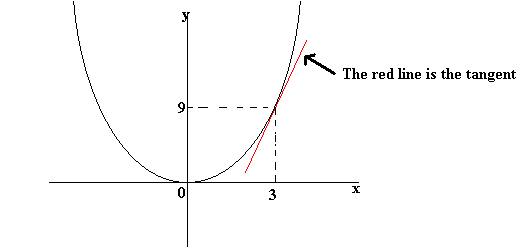
\includegraphics[width=\textwidth]{gradient}
		\end{column}
	\end{columns}
	\begin{itemize}
		\pause\item Equivalent to the \textbf{gradient} of a graph, $\dfrac{\text{change in } y}{\text{change in } x}$		
		\pause\item For moving objects:
		\begin{itemize}
			\pause\item \textbf{Velocity} is the derivative of \textbf{displacement}
			\pause\item \textbf{Acceleration} is the derivative of \textbf{velocity}
			\pause\item NB \textbf{speed} is the \textbf{magnitude} of velocity
		\end{itemize}
	\end{itemize}
\end{frame}

\begin{frame}{Calculus: integration}
	\begin{itemize}
		\pause\item The opposite of differentiation: $x$ is the \textbf{integral} of $\dfrac{dx}{dt}$
		\pause\item We are interested in \textbf{numerical integration}, i.e. by computer calculation
		\pause\item \textbf{Euler method}: given $x$ and $\frac{dx}{dt}$ at time $t$, we can \textbf{estimate} the value of $x$ at time $t+h$:
	\end{itemize}
	\begin{columns}
		\begin{column}{0.58\textwidth}
			\pause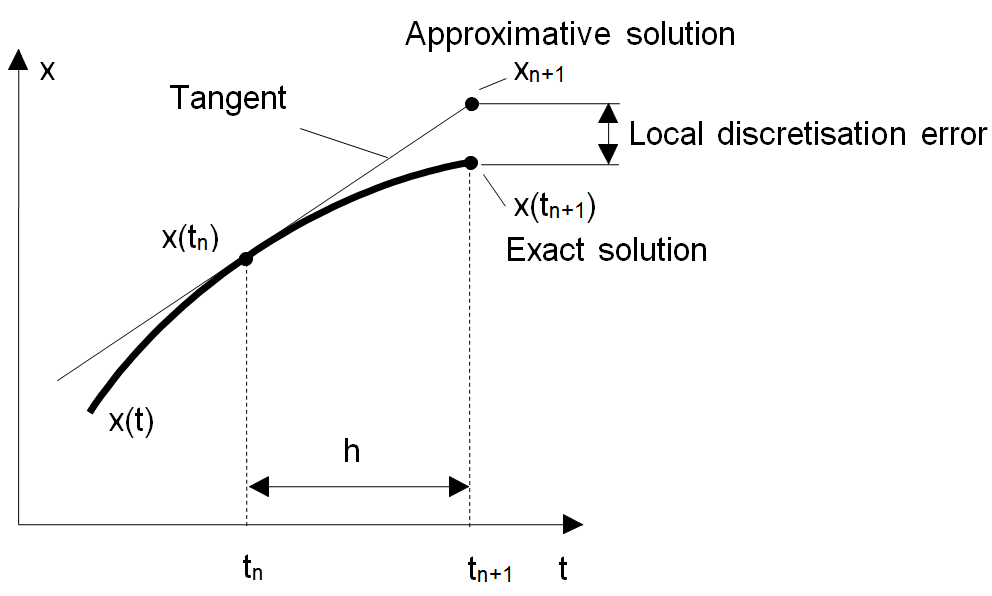
\includegraphics[width=\textwidth]{euler_method}
		\end{column}
		\begin{column}{0.4\textwidth}
			\pause $$ x(t+h) \approx x(t) + h \times \frac{dx}{dt}(t) $$
		\end{column}
	\end{columns}
\end{frame}

\begin{frame}{Basic simulation loop}
	\begin{itemize}
		\pause\item For each object, store its position $\boldsymbol{x}$ and velocity $\boldsymbol{v}$
		\pause\item On each time step $\Delta{t}$:
		\begin{itemize}
			\pause\item Find the new position using numerical integration, $\boldsymbol{x}' = \boldsymbol{x} + $$\boldsymbol{v}\Delta{t}$
			\pause\item Calculate the forces acting on the object, and thus the acceleration $\boldsymbol{a}$ from Newton's second law, $\boldsymbol{F} = m\boldsymbol{a}$
			\pause\item Find the new velocity using numerical integration, $\boldsymbol{v}' = \boldsymbol{v} + $$\boldsymbol{a}\Delta{t}$
		\end{itemize}
	\end{itemize}
\end{frame}

\begin{frame}{Newton's Laws of Motion}
	\begin{center}
		\pause An object remains at rest or moves at constant velocity unless acted upon by an external force
		
		\vspace{2ex}
		
		\pause $\boldsymbol{F} = m\boldsymbol{a}$: The sum of forces acting upon an object is equal to its mass multiplied by its acceleration
		
		\vspace{2ex}
		
		\pause When one body exerts a force on another, the second body exerts an equal and opposite force on the first
	\end{center}
\end{frame}

\begin{frame}{Basic collision response}
	\begin{columns}
		\begin{column}{0.4\textwidth}
			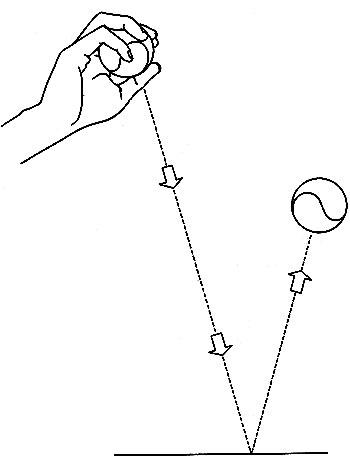
\includegraphics[width=\textwidth]{bounce_reflection}
		\end{column}
		\begin{column}{0.58\textwidth}
			\begin{itemize}
				\pause\item For an \textbf{elastic collision}, the component of velocity parallel to the \textbf{surface normal}
					is \textbf{reversed}
				\pause\item E.g.\ if the surface is the $xz$ plane, flip the $y$ component
				\pause\item For an \textbf{inelastic collision}, some velocity is lost
				\pause\item Flip the $y$ component and multiply it by something between $0$ and $1$
			\end{itemize}
		\end{column}
	\end{columns}
\end{frame}


\part{Skeletal Animation}
\frame{\partpage}

\begin{frame}{Coordinate spaces}
	\begin{center}
		\begin{tabular}{cl}
			\pause Model space \\
			\pause $\downarrow$ & Model matrix \\
			\pause World space \\
			\pause $\downarrow$ & View matrix \\
			\pause Camera space \\
			\pause $\downarrow$ & Projection matrix \\
			\pause Screen space
		\end{tabular}
	\end{center}
\end{frame}

\begin{frame}{Rule of thumb}
	\begin{itemize}
		\pause\item When performing calculations, \textbf{do not mix} vectors from \textbf{different coordinate spaces}
		\pause\item E.g.\ when performing lighting calculations, ensure your fragment position, normal, light direction, eye direction are all
			in the \textbf{same} space
	\end{itemize}
\end{frame}

\begin{frame}{Scene graph}
	\begin{itemize}
		\pause\item It is often useful to organise objects into a \textbf{hierarchy}
		\pause\item Each node in the hierarchy has its own model matrix
		\pause\item Transformations stack: object is affected by its own transformation,
			and that of its parent,
			and that of its grandparent,
			and so on
		\pause\item The model matrix is the \textbf{product} of model matrices for the node and its ancestors
	\end{itemize}
\end{frame}


\begin{frame}{Rigging}
	\begin{columns}
		\begin{column}{0.4\textwidth}
			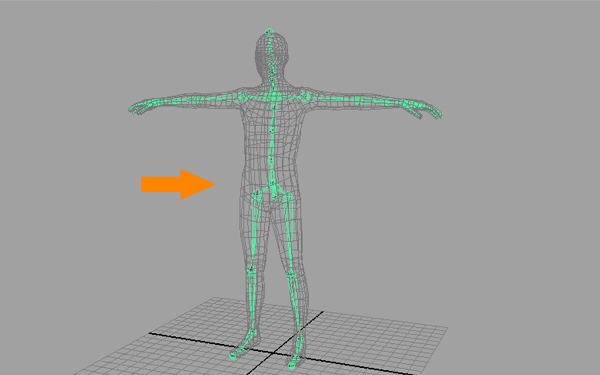
\includegraphics[width=\textwidth]{human_rig}
		\end{column}
		\begin{column}{0.58\textwidth}
			\begin{itemize}
				\pause\item A \textbf{skeleton} is composed of \textbf{bones}
				\pause\item Arranged in a \textbf{hierarchy}
				\pause\item Each bone is essentially just a \textbf{transformation}
					\begin{itemize}
						\pause\item Usually just rotation around a pivot point
						\pause\item 3D modelling software often represents bones as lines from parent bone to child bone
					\end{itemize}
			\end{itemize}
		\end{column}
	\end{columns}
\end{frame}

\begin{frame}{Keyframe animation}
	\begin{itemize}
		\pause\item Most basic form of skeletal animation: specify bone transformations for each frame of animation
		\pause\item ... or just for \textbf{keyframes} and interpolate between them
		\pause\item Keyframes set up by an animator, through motion capture, or a combination of the two
		\pause\item More advanced: can \textbf{blend} animations
			\begin{itemize}
				\pause\item E.g.\ blend between walking and running
				\pause\item E.g.\ bottom half plays ``walk'' animation, top half plays ``fire weapon'' animation
			\end{itemize}
	\end{itemize}
\end{frame}

\begin{frame}{Forward kinematics (FK)}
	\begin{columns}
		\begin{column}{0.4\textwidth}
			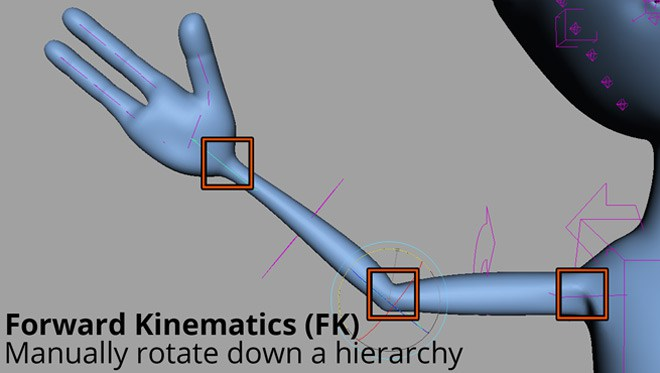
\includegraphics[width=\textwidth]{forward_kinematics}
		\end{column}
		\begin{column}{0.58\textwidth}
			\begin{itemize}
				\pause\item Bone transformations are set \textbf{explicitly}
				\pause\item Children are affected by parent transformations,
					e.g.\ if upper arm rotates, lower arm rotates with it
			\end{itemize}
		\end{column}
	\end{columns}
\end{frame}

\begin{frame}{Inverse kinematics (IK)}
	\begin{columns}
		\begin{column}{0.4\textwidth}
			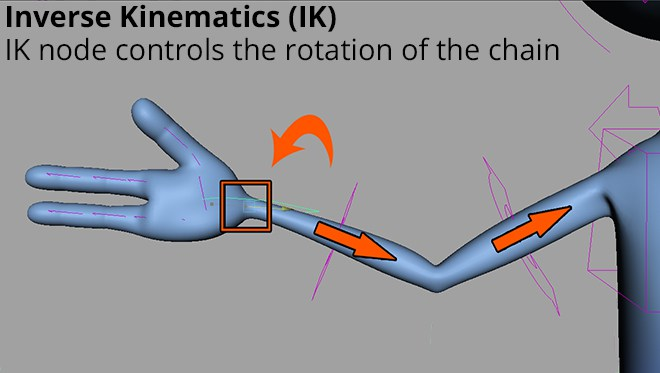
\includegraphics[width=\textwidth]{inverse_kinematics}
		\end{column}
		\begin{column}{0.58\textwidth}
			\begin{itemize}
				\pause\item Bone transformations are calculated to reach a \textbf{target}
				\pause\item E.g.\ we want character's hand to touch an object; IK calculates rotations of upper and lower arm to achieve this
					subject to constraints
			\end{itemize}
		\end{column}
	\end{columns}
\end{frame}

\begin{frame}{The most common use for IK}
	\begin{center}
		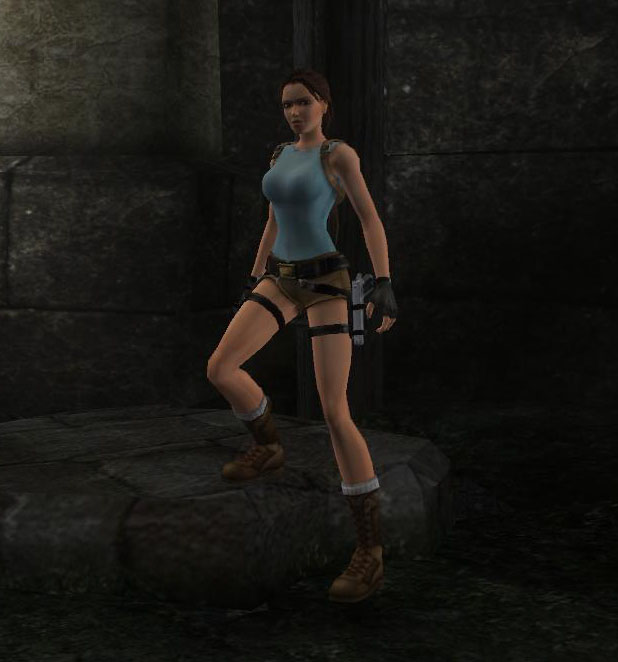
\includegraphics[height=0.4\textheight]{ik_feet3} \quad
		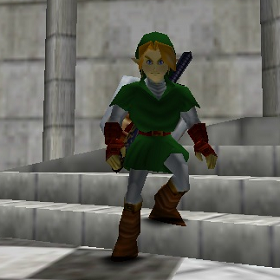
\includegraphics[height=0.4\textheight]{ik_feet2}
		
		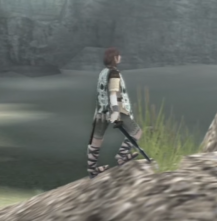
\includegraphics[height=0.4\textheight]{ik_feet4} \quad
		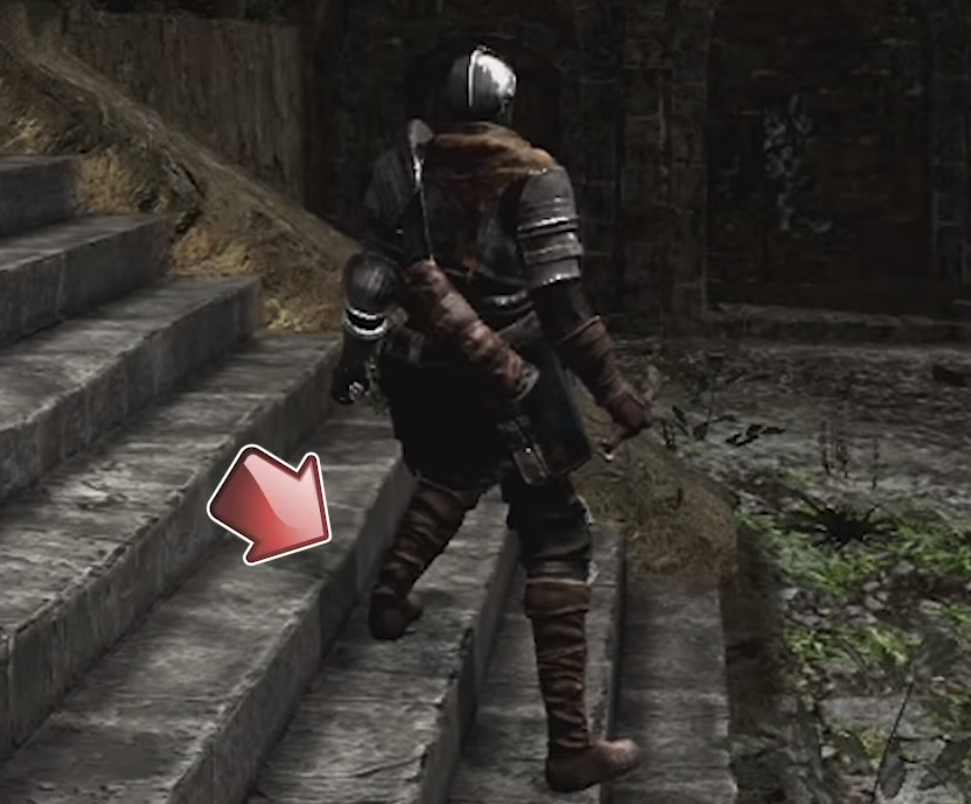
\includegraphics[height=0.4\textheight]{ik_feet}
	\end{center}
\end{frame}

\begin{frame}{Ragdolls}
	\begin{columns}
		\begin{column}{0.4\textwidth}
			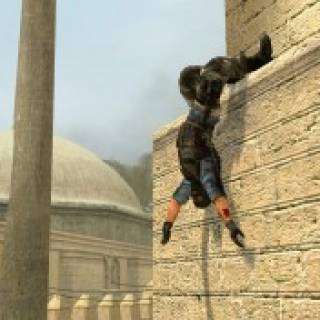
\includegraphics[width=\textwidth]{ragdoll}
		\end{column}
		\begin{column}{0.58\textwidth}
			\begin{itemize}
				\pause\item Attach a \textbf{rigid body} to each bone and run a \textbf{physics simulation}
				\pause\item Often used for death animations
				\pause\item Many games mix and blend some or all of keyframe animation, IK, and physics simulation
			\end{itemize}
		\end{column}
	\end{columns}
\end{frame}

\begin{frame}{Skinning}
	\begin{itemize}
		\pause\item The character is animated by changing the bone transformations
		\pause\item \textbf{Skinning} is the process of applying these transformations to the vertices of the model
		\pause\item Generally handled by a \textbf{vertex shader}
		\pause\item Uses \textbf{bone weights} to specify how much each vertex is affected by each bone's transformation
	\end{itemize}
\end{frame}

\begin{frame}{Bone weights}
	\begin{columns}
		\begin{column}{0.4\textwidth}
			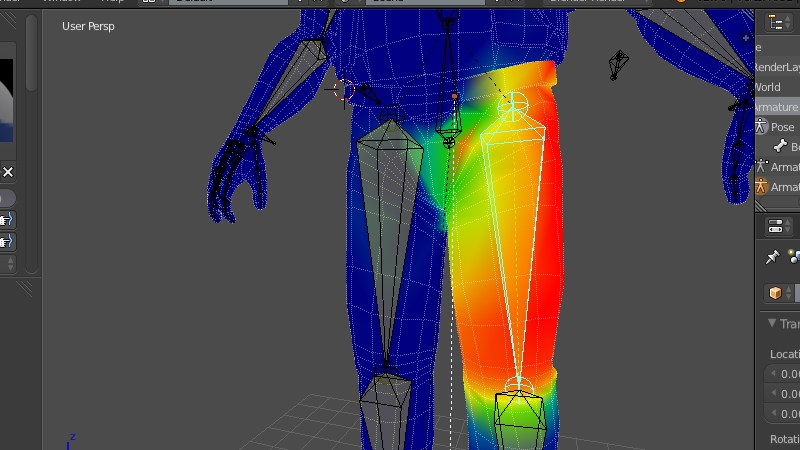
\includegraphics[width=\textwidth]{bone_weights}
		\end{column}
		\begin{column}{0.58\textwidth}
			\begin{itemize}
				\pause\item Each vertex in the model has a list of \textbf{bone weights}
				\pause\item Usually ``painted'' onto the model by the 3D artist
				\pause\item Vertex position is calculated as a weighted average of joint transforms
			\end{itemize}
		\end{column}
	\end{columns}
\end{frame}

\begin{frame}{Secondary effects}
	\begin{itemize}
		\pause\item Additional movement that occurs as a result of the skeletal animation
		\pause\item For example: swinging clothes or hair, jiggle of body parts, skin sliding over bones
		\pause\item Can be \textbf{simulated} using a variety of techniques, though this is often expensive even for simplified methods
		\pause\item A popular approach is to use \textbf{morph targets} (aka \textbf{blend shapes})
	\end{itemize}
\end{frame}

\begin{frame}{Morph targets}
	\begin{itemize}
		\pause\item Take two (or more) \textbf{topologically identical} meshes (i.e. the same vertices in the same order)
		\pause\item Deform each mesh to represent a different \textbf{target}, e.g. happy, sad, angry, neutral
		\pause\item Create effects by \textbf{interpolating} the vertex positions to blend between the targets
	\end{itemize}
	\begin{figure}[h!]
		\pause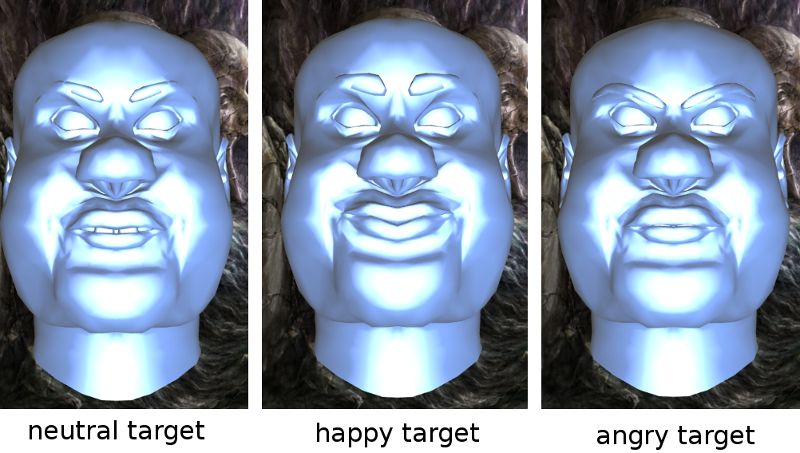
\includegraphics[width=0.4\textwidth]{morph_targets}
		\caption*{Image source: \url{https://antongerdelan.net/opengl/blend_shapes.html}}
	\end{figure}
\end{frame}


\begin{frame}{Next steps}
	\begin{itemize}
		\item \textbf{Review} the additional asynchronous material for more background on physics and animation techniques.
		\item \textbf{Attend} the workshop to learn how to use the Bullet Physics library in your own applications.
	\end{itemize}
\end{frame}

\end{document}

